% ============================================================
% CHAPTER 13 — AGING AND STATE OF HEALTH (SOH) TRACKING
% ============================================================

\chapter{Aging and State of Health (SOH) Tracking}
\label{ch:soh_tracking}

\section{Introduction: The Moving Target of Battery Health}
\label{sec:13_intro}

The estimation algorithms developed in Chapters~5 through~9 primarily focus on tracking fast-transient states, most notably the State of Charge (SOC). However, a battery is an electrochemically active system that fundamentally degrades over time. Parameters that are considered constant during a single drive cycle—such as the total charge capacity ($Q_n$) and the baseline ohmic resistance ($R_0$)—drift significantly over months and years of operation.

State of Health (SOH) tracking is the process of quantifying this slow degradation. Accurate SOH estimation is critical for ensuring operational safety, predicting the Remaining Useful Life (RUL) of the pack, and updating the baseline parameters used by the SOC estimators. If a BMS assumes a battery retains its factory-nominal capacity when it has actually degraded by 20\%, the resulting SOC and driving range predictions will be dangerously inaccurate.

This chapter details the physical mechanisms of battery aging, establishes the mathematical definitions of SOH, and explores the algorithmic frameworks—such as Dual-Time-Scale Observers, empirical capacity-fade modeling, and Differential Curve Analysis—required to estimate degradation in real time and to project it forward into a meaningful Remaining Useful Life prediction.

\subsection{Why SOH Is Harder Than SOC}
\label{subsec:13_why_hard}

It is worth pausing to articulate precisely why SOH estimation is treated as a distinct, and in many ways harder, problem than SOC estimation, rather than simply "the same Kalman filter run more slowly."

\begin{enumerate}
    \item \textbf{No direct sensor exists.} SOC, while not directly measurable either, has a comparatively strong and well-characterized relationship to open-circuit voltage. SOH parameters such as $Q_n$ and $R_0$ must be inferred from how the cell \emph{responds} to excitation, which requires either a full characterization cycle or a carefully designed partial-cycle inference scheme.
    \item \textbf{The signal-to-noise ratio is unfavorable.} Capacity typically fades by only a fraction of a percent per week of normal use. Distinguishing this genuine, slow trend from ordinary measurement noise, sensor drift, and temperature-driven short-term variation is a fundamentally difficult signal processing problem.
    \item \textbf{The ground truth is expensive to obtain.} Validating an SOH estimate against a true reference requires a full, controlled reference performance test (RPT) — a slow, low-rate, temperature-controlled charge/discharge cycle performed in a laboratory setting — which is impractical to perform routinely on a vehicle in the field. Online SOH algorithms must therefore be validated primarily through modeling and periodic (not continuous) ground-truth checks.
\end{enumerate}

\begin{figure}[htbp]
\centering
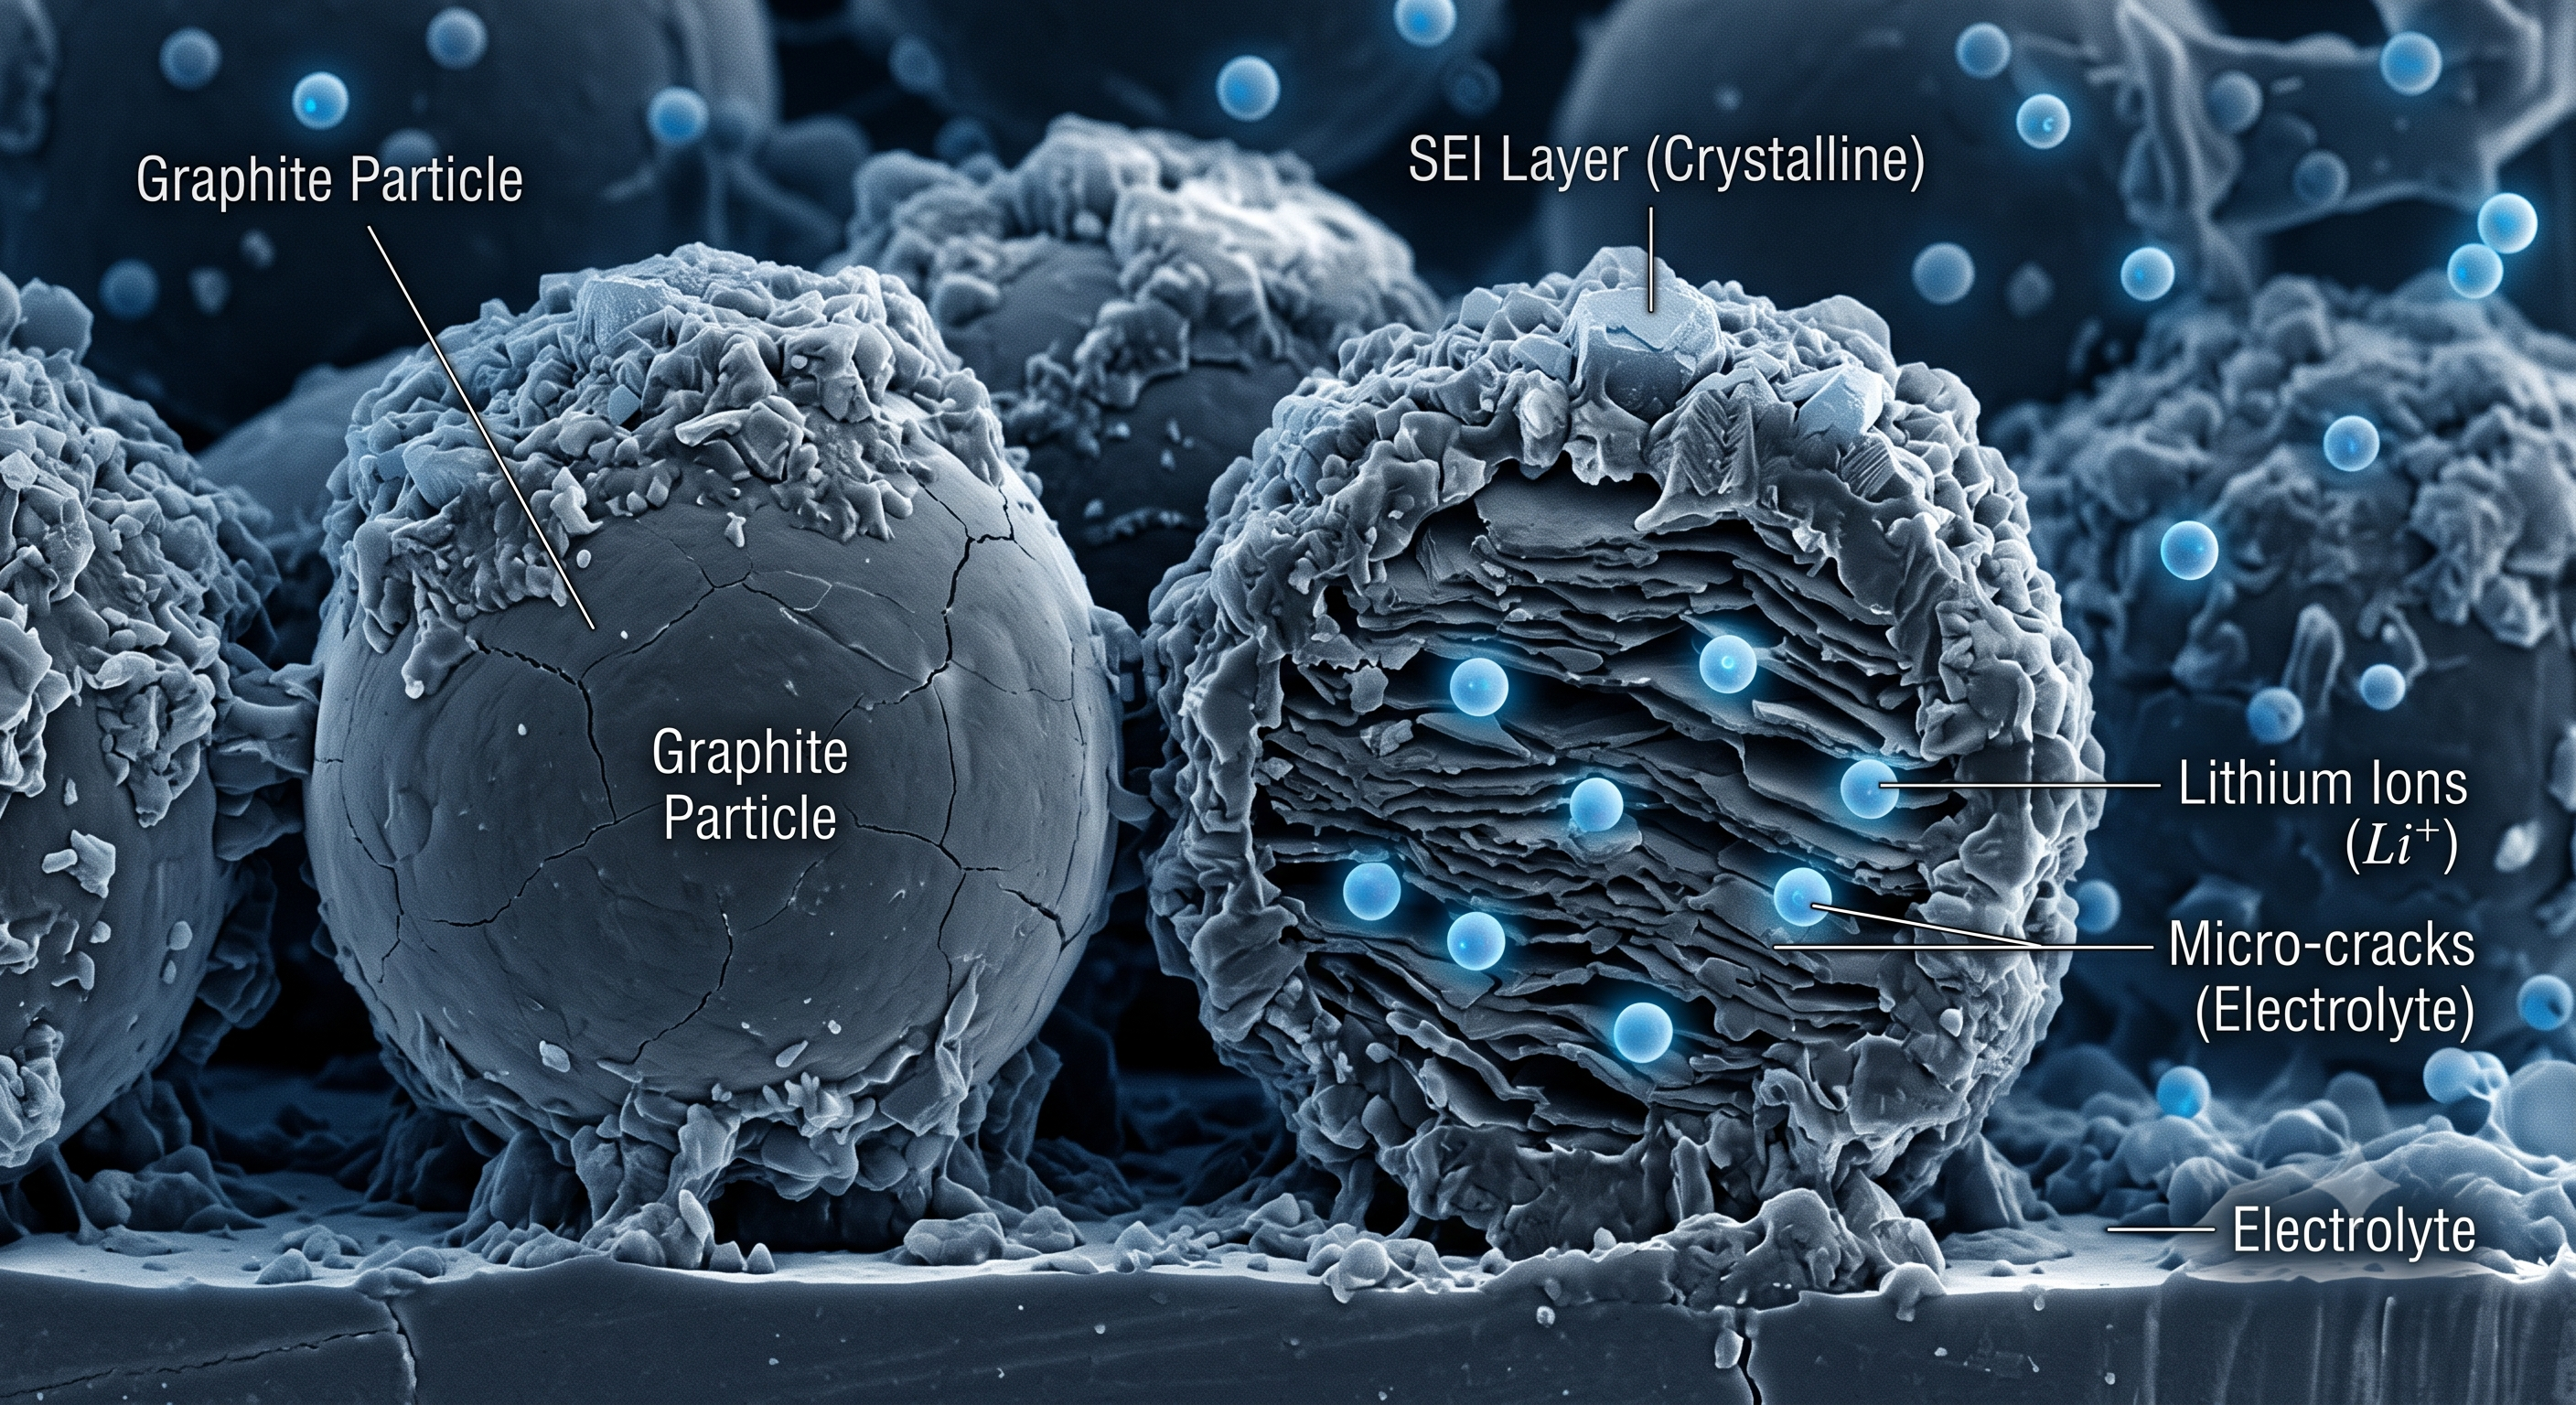
\includegraphics[width=0.65\textwidth]{Ch-9-2.png}
\caption{Conceptual illustration of the timescale separation between SOC dynamics and SOH degradation.}
\label{fig:13_timescale_placeholder}
\end{figure}

% ============================================================
\section{Physical Mechanisms of Degradation}
\label{sec:13_mechanisms}

Battery degradation is not caused by a single phenomenon, but rather by a complex web of coupled chemical and mechanical stress factors. These aging mechanisms are broadly categorized into two primary modes: Loss of Lithium Inventory and Loss of Active Material, with a third, closely related category — conductivity loss — often treated separately due to its distinct signature.

\subsection{Loss of Lithium Inventory (LLI)}
\label{subsec:13_lli}

LLI occurs when cyclable lithium ions ($\text{Li}^+$) are permanently consumed by parasitic side reactions and are no longer available to shuttle between the anode and cathode. The most dominant cause of LLI is the continuous growth of the \textbf{Solid Electrolyte Interphase (SEI)} layer on the graphite anode. While an initial SEI layer is necessary for battery stability, it continually thickens over the battery's lifespan, trapping lithium ions and consuming electrolyte. LLI directly manifests as \textbf{capacity fade}.

A second, more dangerous contributor to LLI is \textbf{lithium plating}: under conditions of low temperature, high charge rate, or high SOC, lithium ions may deposit as metallic lithium on the anode surface rather than intercalating properly into the graphite structure. Plated lithium is largely unrecoverable and, beyond its contribution to capacity fade, poses a distinct safety hazard, since metallic lithium deposits can grow into dendritic structures capable of piercing the separator and causing an internal short circuit. This is one of the key reasons production BMS designs impose conservative charge-current limits at low temperatures, well below what the cell could otherwise tolerate from a pure thermal standpoint.

\subsection{Loss of Active Material (LAM)}
\label{subsec:13_lam}

LAM refers to the physical degradation of the electrode structures. During charging and discharging, the intercalation of lithium ions causes the electrode particles to expand and contract. Over thousands of cycles, this mechanical stress leads to particle micro-cracking, binder decomposition, and electrical isolation of active material. LAM drives \textbf{internal resistance growth} and reduces the cell's power capability.

LAM is further subdivided in the literature into LAM at the negative electrode (LAM$_{\text{NE}}$) and LAM at the positive electrode (LAM$_{\text{PE}}$), since the two electrodes typically degrade via different mechanisms and at different rates. Positive electrode degradation is commonly driven by transition metal dissolution (particularly in NMC and NCA chemistries), in which manganese, nickel, or cobalt ions dissolve out of the cathode lattice, migrate across the separator, and deposit on the anode, where they catalyze further SEI growth — a cross-coupling effect that links positive-electrode LAM back to negative-electrode LLI.

\subsection{Conductivity Loss}
\label{subsec:13_conductivity}

A third contributor, often lumped together with LAM in simplified treatments but worth distinguishing, is the loss of electrical and ionic conductivity within the cell that is not attributable to material loss per se. This includes electrolyte dry-out or decomposition (reducing ionic conductivity between electrodes), corrosion of current collectors, and degradation of conductive carbon additives within the electrode composite. Conductivity loss manifests primarily as an increase in the cell's ohmic resistance $R_0$ and, in severe cases, can produce a rapid, nonlinear "knee point" in the resistance-growth trajectory late in life (see Section~\ref{subsec:13_knee_point}).

\begin{table}[htbp]
\centering
\caption{Summary of primary lithium-ion degradation mechanisms.}
\label{tab:13_aging_mechanisms}
\renewcommand{\arraystretch}{1.4}
\begin{tabularx}{\textwidth}{@{}l X X@{}}
\toprule
\textbf{Degradation Mode} & \textbf{Physical Root Causes} & \textbf{Observable Effect} \\
\midrule
\textbf{LLI (Lithium Loss)} & SEI layer growth; Lithium plating during low-temperature fast charging. & Decrease in total usable capacity ($Q_n$). \\
\textbf{LAM (Material Loss)} & Particle micro-cracking; Transition metal dissolution; Binder failure. & Increase in ohmic ($R_0$) and polarization ($R_1$) resistance. \\
\textbf{Conductivity Loss} & Electrolyte depletion/dry-out; Current collector corrosion; Conductive additive breakdown. & Severe impedance rise and power fade, often nonlinear late in life. \\
\bottomrule
\end{tabularx}
\end{table}

\subsection{Stress Factors Governing Degradation Rate}
\label{subsec:13_stress_factors}

The mechanisms above do not proceed at a fixed rate; their kinetics are strongly modulated by four primary operating stress factors, summarized in Table~\ref{tab:13_stress_factors}. Understanding these stress factors is essential background for the empirical fade models introduced in Section~\ref{sec:13_fade_models}, since virtually every practical capacity-fade model is parameterized directly in terms of them.

\begin{table}[htbp]
\centering
\caption{Primary operating stress factors influencing degradation rate.}
\label{tab:13_stress_factors}
\renewcommand{\arraystretch}{1.4}
\begin{tabularx}{\textwidth}{@{}l X@{}}
\toprule
\textbf{Stress Factor} & \textbf{Effect on Degradation} \\
\midrule
Temperature & Accelerates SEI growth and side reactions per Arrhenius kinetics (Chapter~14, Eq.~14.1); also elevates lithium plating risk at low temperatures. \\
State of Charge (calendar) & High storage SOC accelerates parasitic side reactions and electrolyte oxidation at the cathode. \\
Depth of Discharge (DoD) & Larger DoD swings increase mechanical strain and particle cracking per cycle. \\
C-rate (charge/discharge current) & High C-rate charging increases plating risk and local current density hotspots; high C-rate discharge increases Joule heating. \\
\bottomrule
\end{tabularx}
\end{table}

\begin{figure}[htbp]
\centering
\includegraphics[width=0.65\textwidth]{Ch-9-2-1.png}
\caption{Conceptual sensitivity of capacity fade rate to the four dominant stress factors.}
\label{fig:13_stress_factor_placeholder}
\end{figure}

% ============================================================
\section{Mathematical Definitions of SOH}
\label{sec:13_soh_math}

Because degradation affects both energy storage and power delivery, SOH is typically defined along two distinct axes: Capacity-based SOH and Resistance-based SOH.

\subsection{Capacity-Based SOH ($SOH_C$)}
\label{subsec:13_sohc}

$SOH_C$ quantifies the remaining energy storage capability of the battery, which directly translates to the driving range of an electric vehicle. It is defined as the ratio of the currently available maximum capacity to the factory-rated nominal capacity:
\begin{equation}
    SOH_C(t) = \frac{Q_{\text{act}}(t)}{Q_{\text{nom}}} \times 100\%
    \label{eq:13_sohc}
\end{equation}
where $Q_{\text{act}}(t)$ is the actual capacity at time $t$, and $Q_{\text{nom}}$ is the Beginning-of-Life (BOL) capacity. An EV battery is typically considered at its automotive End-of-Life (EOL) when $SOH_C$ reaches 70\% to 80\%.

\subsection{Resistance-Based SOH ($SOH_R$)}
\label{subsec:13_sohr}

$SOH_R$ quantifies the power delivery capability, which impacts vehicle acceleration and regenerative braking efficiency. It is defined based on the growth of internal ohmic resistance:
\begin{equation}
    SOH_R(t) = \frac{R_{\text{EOL}} - R_{\text{act}}(t)}{R_{\text{EOL}} - R_{\text{BOL}}} \times 100\%
    \label{eq:13_sohr}
\end{equation}
where $R_{\text{act}}(t)$ is the current measured resistance, $R_{\text{BOL}}$ is the baseline resistance of a new cell, and $R_{\text{EOL}}$ is the predefined failure threshold (often defined as $2 \times R_{\text{BOL}}$).

\subsection{Reconciling $SOH_C$ and $SOH_R$}
\label{subsec:13_reconciling}

In an ideal, single-mechanism aging scenario, $SOH_C$ and $SOH_R$ would decline in lockstep, and a single scalar SOH value would suffice. In practice, because LLI and LAM/conductivity loss proceed at different relative rates depending on the dominant stress factors a given cell has experienced (Section~\ref{subsec:13_stress_factors}), $SOH_C$ and $SOH_R$ frequently diverge. A cell that has spent most of its life in mild, low-current, temperature-controlled use (e.g., stationary grid storage) will typically show $SOH_C$ declining faster than $SOH_R$, dominated by calendar-driven LLI. Conversely, a cell subjected to frequent high-current fast charging will often show $SOH_R$ declining faster, dominated by LAM and plating-related mechanisms. Because vehicle range depends on $SOH_C$ while acceleration and fast-charge acceptance depend on $SOH_R$, a well-designed BMS reports both quantities to the vehicle's energy management system rather than collapsing them into a single "battery health" number, even though a single number is often what is ultimately displayed to the end user for simplicity.

% ============================================================
\section{Empirical and Semi-Empirical Capacity Fade Models}
\label{sec:13_fade_models}

Before an online estimator can correct its parameters against real-time data, it is useful to have a baseline model of \emph{expected} degradation, both to sanity-check the estimator's output and to extrapolate toward a Remaining Useful Life prediction (Section~\ref{sec:13_rul}). Two complementary modeling philosophies are used in practice: calendar-aging models and cycle-aging models, which are typically combined additively.

\subsection{Calendar Aging}
\label{subsec:13_calendar_aging}

Calendar aging refers to capacity loss that accrues purely from the passage of time, independent of cycling, and is dominated by parasitic side reactions at the electrode-electrolyte interface. A widely used empirical form, motivated by diffusion-limited SEI growth, expresses calendar fade as proportional to the square root of elapsed time:
\begin{equation}
    Q_{\text{loss,cal}}(t) = A_{\text{cal}}(T, SOC) \cdot \sqrt{t}
    \label{eq:13_calendar_fade}
\end{equation}
where $A_{\text{cal}}(T, SOC)$ is a pre-exponential coefficient that itself depends on storage temperature and storage SOC (typically via an Arrhenius-type temperature dependence combined with an exponential or polynomial SOC dependence, fitted from accelerated aging test data).

\subsection{Cycle Aging}
\label{subsec:13_cycle_aging}

Cycle aging refers to the additional capacity loss attributable specifically to charge/discharge cycling, superimposed on top of the calendar-aging baseline. A common empirical form expresses cycle fade as a power-law function of the total ampere-hour throughput $Ah_{\text{total}}$ (the cumulative charge that has passed through the cell, summed across both charge and discharge, sometimes called the "throughput" or "Wöhler" model by analogy to metal fatigue curves):
\begin{equation}
    Q_{\text{loss,cyc}} = B_{\text{cyc}}(T, \text{DoD}, C_{\text{rate}}) \cdot Ah_{\text{total}}^{\,z}
    \label{eq:13_cycle_fade}
\end{equation}
where $z$ is typically found empirically to lie in the range of 0.5–0.7 for many lithium-ion chemistries (again reflecting an underlying diffusion-limited process), and $B_{\text{cyc}}$ is a coefficient fitted from cycling test data at various combinations of temperature, DoD, and C-rate.

\subsection{Combined Fade Model}
\label{subsec:13_combined_fade}

The two contributions are commonly combined additively, under the simplifying (and not universally accurate) assumption that calendar and cycle aging mechanisms act independently:
\begin{equation}
    Q_{\text{loss,total}}(t) = Q_{\text{loss,cal}}(t) + Q_{\text{loss,cyc}}\big(Ah_{\text{total}}(t)\big)
    \label{eq:13_combined_fade}
\end{equation}
This additive decomposition is popular precisely because it allows a fleet-management system to separately attribute observed fade to "how long the battery has existed" versus "how hard the battery has been used," which is operationally useful for warranty analysis, but the assumption of independence breaks down as the cell approaches its knee point (Section~\ref{subsec:13_knee_point}), where calendar- and cycle-driven mechanisms increasingly interact.

\subsection{The Knee Point and Nonlinear Late-Life Fade}
\label{subsec:13_knee_point}

Both Equations~\ref{eq:13_calendar_fade} and~\ref{eq:13_cycle_fade} describe smooth, gradually decelerating fade trajectories (due to the square-root and sub-linear power-law forms). In practice, however, many cells exhibit a distinct \textbf{knee point}: a period of relatively slow, near-linear fade followed by an abrupt transition to a much steeper, sometimes near-exponential decline. The physical origin of the knee point is generally attributed to a self-reinforcing interaction between mechanisms — for example, LAM-driven resistance growth increases local current density and heating, which accelerates further lithium plating and SEI growth, which in turn accelerates LAM, in a runaway feedback loop analogous to the thermal feedback discussed in Chapter~14. Because the empirical models of Equations~\ref{eq:13_calendar_fade}–\ref{eq:13_cycle_fade} are fitted primarily from pre-knee data (since post-knee data is by definition close to end-of-life and less abundant in test datasets), naive extrapolation of these models can significantly \emph{underestimate} late-life fade rate, which is one of the most active areas of research in battery prognostics today.

\begin{figure}[htbp]
\centering
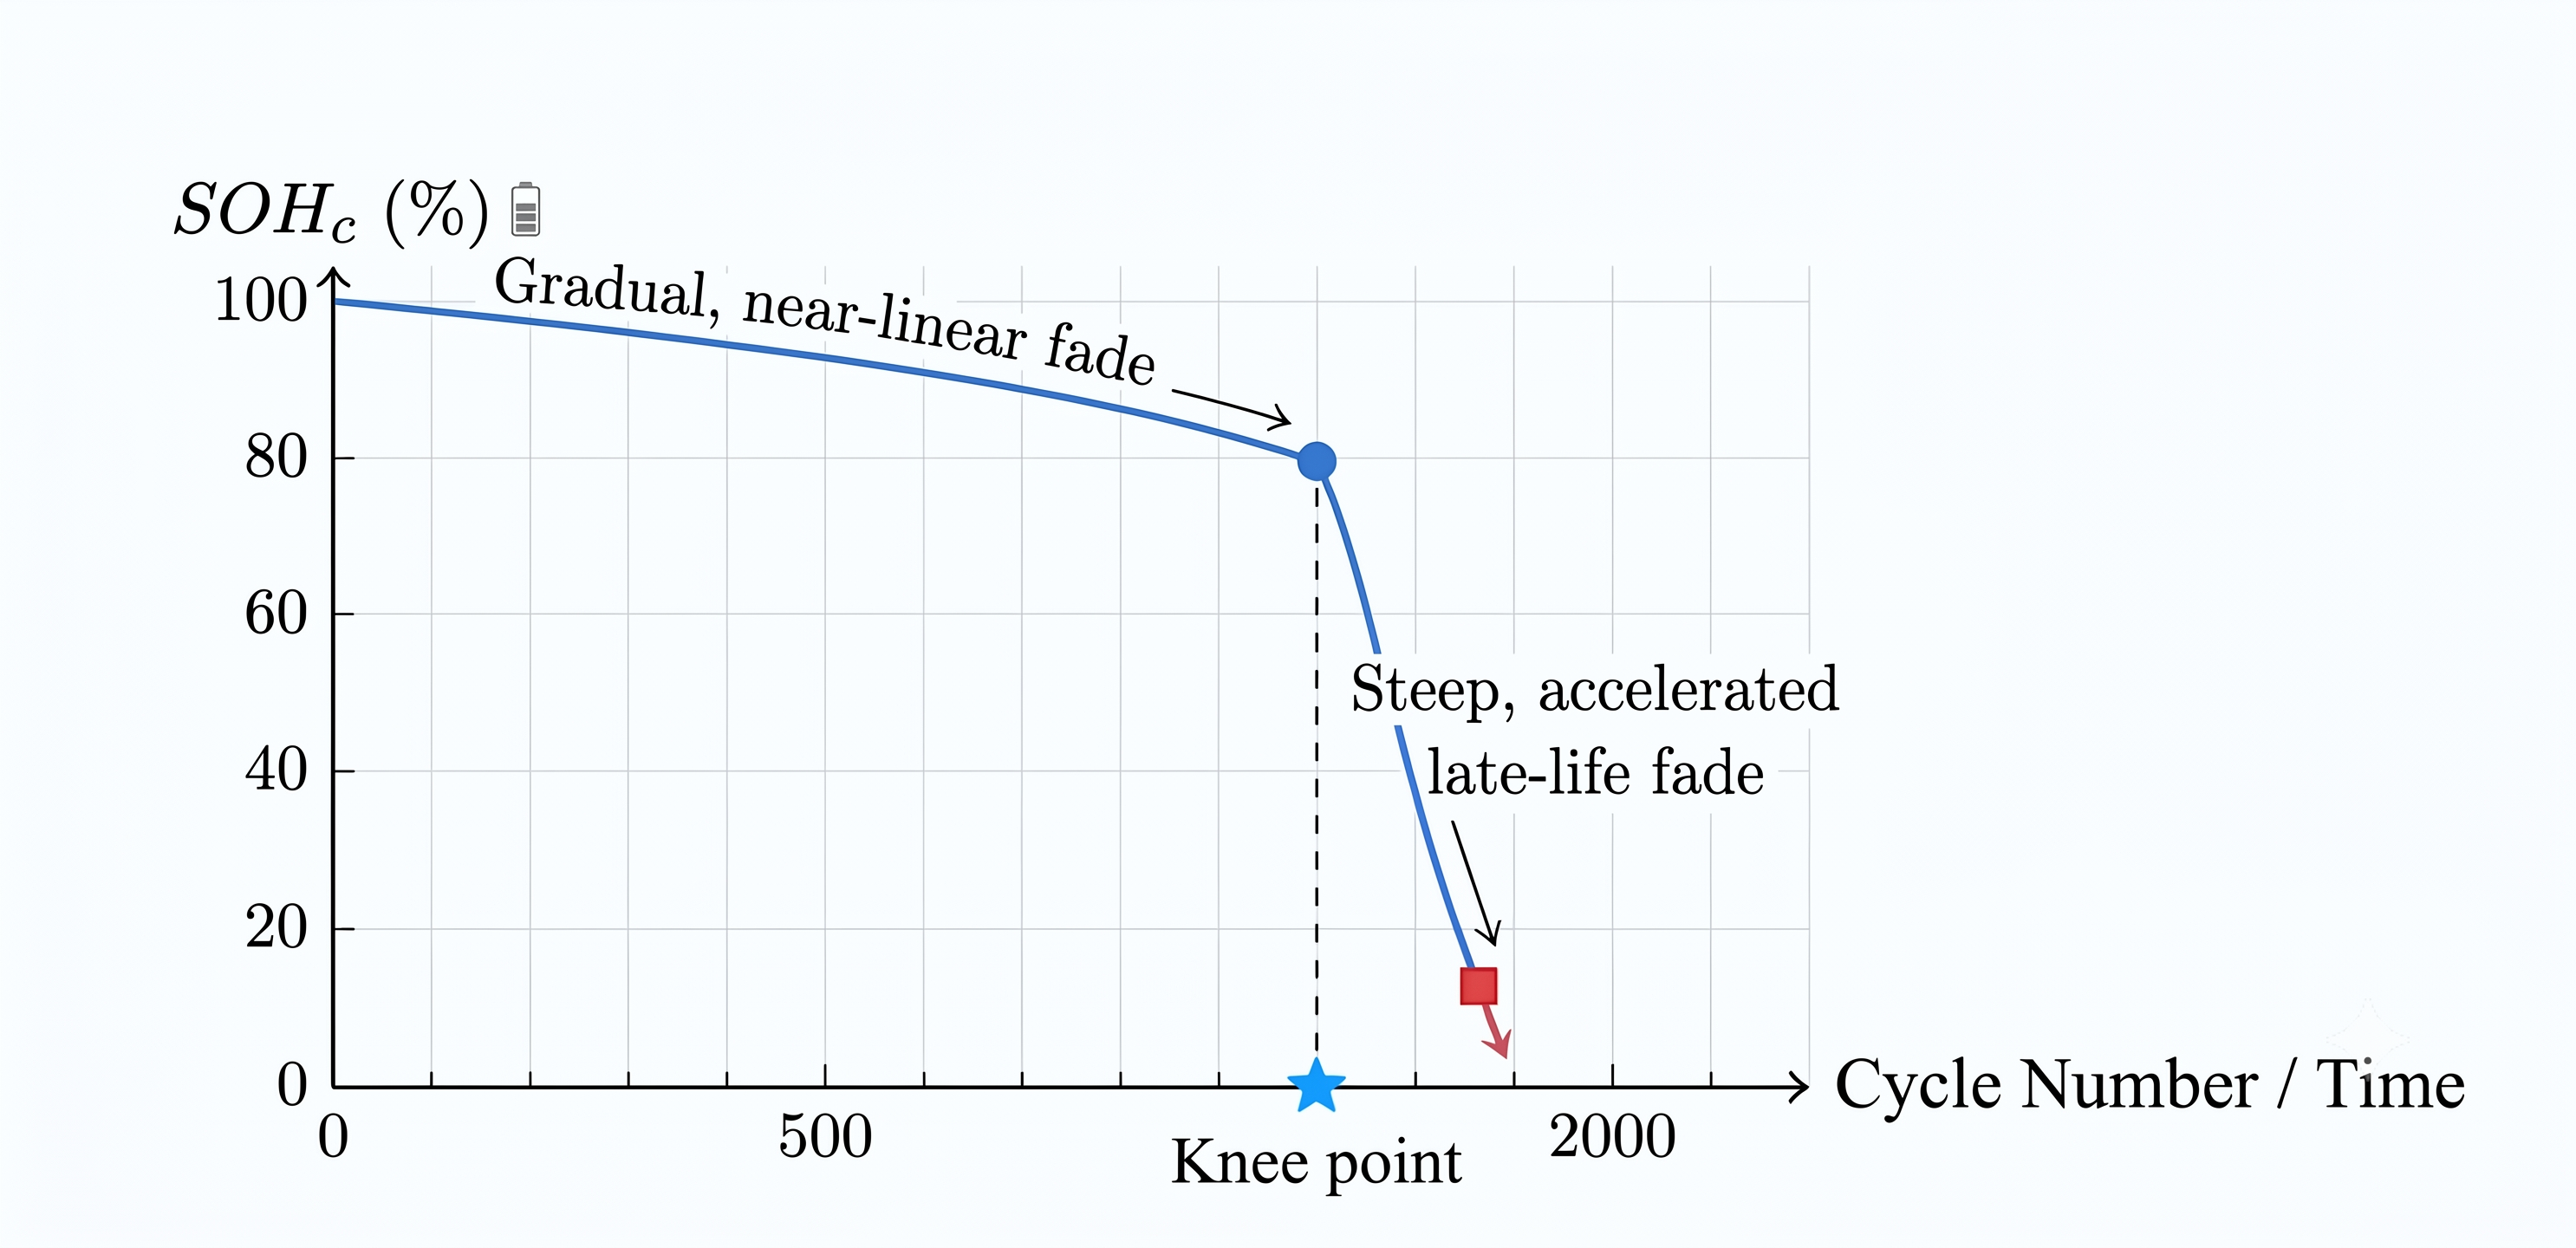
\includegraphics[width=0.65\textwidth]{chapter11-1.png}
\caption{Conceptual illustration of knee-point behavior in a capacity fade trajectory.}
\label{fig:13_knee_point}
\end{figure}

% ============================================================
\section{The Dual-Time-Scale Estimation Problem}
\label{sec:13_dual_time_scale}

Estimating both SOC and SOH simultaneously presents a severe mathematical challenge due to scale separation. SOC changes rapidly (over minutes and seconds) driven by the current $I(t)$. Conversely, SOH changes glacially (over months and years).

If a single Extended Kalman Filter (EKF) attempts to estimate both the fast states ($z$) and the slow parameters ($Q_n$, $R_0$) simultaneously in a single state vector, the filter becomes highly susceptible to cross-interference. Measurement noise will incorrectly manifest as parameter drift, causing numerical instability.

\subsection{Dual Extended Kalman Filter (DEKF)}
\label{subsec:13_dekf}

To resolve this, modern BMS architectures use a \textbf{Dual-Time-Scale Observer}. The system is decoupled into two parallel filters that run at entirely different frequencies:

\begin{enumerate}
    \item \textbf{The State Filter (Fast):} Runs at a high frequency (e.g., 10~Hz). It treats the ECM parameters ($R_0, R_1, C_1, Q_n$) as constants and focuses exclusively on tracking the rapid changes in SOC and polarization voltages.
    \item \textbf{The Parameter Filter (Slow):} Runs at a low frequency (e.g., 0.01~Hz or once per charge cycle). It observes the long-term prediction errors of the State Filter and slowly updates the ECM parameters using a random-walk model: $\theta_{k+1} = \theta_k + r_k$.
\end{enumerate}

By feeding the updated parameters from the Slow Filter back into the Fast Filter, the BMS maintains accuracy over the entire lifespan of the battery without succumbing to high-frequency noise.

\subsection{Why the Random-Walk Parameter Model Is Appropriate}
\label{subsec:13_random_walk}

At first glance, modeling a physically-driven, monotonically-progressing quantity like $Q_n$ as a random walk (Section~\ref{subsec:13_dekf}) seems like a crude simplification — real capacity fade is neither random nor, in the short term, walking in both directions. The justification is more subtle: the random-walk model is not intended to describe the \emph{true underlying physics} of degradation (that is the job of the fade models in Section~\ref{sec:13_fade_models}); it is intended to describe the estimator's \emph{uncertainty} about the parameter between updates. Because the true fade rate is slow and the physical fade models are only approximately correct, allowing the Kalman parameter-filter process noise covariance $Q_\theta$ to inject a small amount of "wandering room" around the physical model's prediction lets the filter track real cells whose degradation deviates from the idealized model, without over-fitting to short-term voltage noise. In practice, the process noise covariance $Q_\theta$ is deliberately tuned to be extremely small relative to the measurement noise covariance $R$, which is precisely what enforces the "glacially slow" update behavior described qualitatively above.

\subsection{Practical Convergence Requirements: Persistent Excitation}
\label{subsec:13_persistent_excitation}

A subtlety that is easy to overlook in a purely equation-driven treatment of the DEKF is that the Parameter Filter can only converge to a meaningful estimate of $Q_n$ and $R_0$ if the input data contains sufficient \textbf{persistent excitation} — that is, sufficient variation in current and SOC operating point to make the parameters observable. A vehicle sitting in traffic at a near-constant, low current provides very little information about $R_0$ (since the ohmic voltage drop $I R_0$ is small and roughly constant) and essentially no information about $Q_n$ (since $Q_n$ is only observable through integrated charge over a meaningfully large SOC excursion). Production implementations typically gate parameter updates behind an excitation-quality check — for example, requiring a minimum SOC swing and a minimum current variance over the averaging window — before allowing the slow filter to update its estimate, to avoid corrupting a good long-term estimate with a poorly-conditioned, noisy update computed from an uninformative driving segment.

% ============================================================
\section{Electrochemical Diagnostics: ICA and DVA}
\label{sec:13_ica_dva}

Beyond adaptive filtering, SOH can be extracted by analyzing the shape of the charging voltage curve. Because the open-circuit voltage ($V_{oc}$) is characterized by flat plateaus where thermodynamic phase transitions occur, tracking shifts in these plateaus reveals deep electrochemical degradation.

\subsection{Incremental Capacity Analysis (ICA)}
\label{subsec:13_ica}

ICA differentiates the charged capacity with respect to the terminal voltage ($dQ/dV$). This mathematical transformation turns flat voltage plateaus into distinct, identifiable peaks.
\begin{equation}
    \text{IC} = \frac{dQ}{dV} \approx \frac{\Delta Q}{\Delta V} = I \cdot \frac{\Delta t}{\Delta V}
    \label{eq:13_ica}
\end{equation}



As the battery ages, the peaks of the IC curve shrink in amplitude (indicating LLI) and shift to higher voltages during charging (indicating ohmic resistance growth). By mapping the area and position of these peaks, algorithms can estimate SOH directly from partial charging events, without requiring a complete 0\% to 100\% charge cycle.

\subsection{Differential Voltage Analysis (DVA)}
\label{subsec:13_dva}

DVA is the complementary transformation to ICA: rather than differentiating capacity with respect to voltage, DVA differentiates voltage with respect to capacity, $dV/dQ$, which is mathematically the inverse of Equation~\ref{eq:13_ica}:
\begin{equation}
    \text{DV} = \frac{dV}{dQ} \approx \frac{\Delta V}{\Delta Q}
    \label{eq:13_dva}
\end{equation}
Where ICA produces sharp peaks at voltage plateaus, DVA produces sharp \emph{troughs} (local minima) at the same underlying phase transitions, since a flat voltage plateau corresponds to a near-zero $dV/dQ$. DVA is often preferred over ICA in practical implementations for one specific reason: because the independent variable in Equation~\ref{eq:13_dva} is capacity (which is measured by integrating current, a comparatively clean, low-noise signal) rather than voltage (which is directly sampled and typically noisier), DVA curves tend to be visibly less noisy than ICA curves computed from the same raw data, at the cost of being somewhat less intuitive to interpret directly.

\subsection{Peak/Trough Tracking and Its Relationship to Electrode-Level SOH}
\label{subsec:13_peak_tracking}

A key strength of both ICA and DVA, beyond providing a single aggregate SOH number, is that with a sufficiently detailed reference model of the cell's open-circuit voltage curve (constructed by combining separately-measured anode and cathode half-cell curves, a technique often called "OCV curve fitting" or "electrode-level modeling"), the position and area of individual IC peaks or DV troughs can, in principle, be mapped back to the specific electrode-level degradation modes discussed in Section~\ref{sec:13_mechanisms} — that is, distinguishing LLI from LAM$_{\text{NE}}$ from LAM$_{\text{PE}}$ from a single voltage curve, without needing to physically disassemble the cell. This technique, sometimes called "degradation mode analysis," is a valuable diagnostic and R\&D tool, though it typically requires higher-fidelity reference curve data and more careful curve-fitting than is practical to run continuously onboard a production vehicle; production BMS implementations of ICA/DVA are therefore usually limited to simpler peak-shift and peak-area heuristics, run periodically (e.g., once per full or near-full charge event) rather than continuously.

\subsection{Practical Implementation Challenges}
\label{subsec:13_ica_challenges}

Despite their elegance, ICA and DVA techniques face several practical obstacles in a real vehicle deployment:

\begin{itemize}
    \item \textbf{Noise sensitivity.} Both transformations involve a numerical derivative, which is inherently noise-amplifying. Production implementations invariably apply a smoothing filter (commonly a Savitzky–Golay filter, chosen for its ability to smooth data while preserving peak shape and position better than a simple moving average) before differentiating.
    \item \textbf{Requirement for consistent excitation conditions.} Because the shape of the OCV curve — and hence the position of IC/DV features — depends weakly on temperature and current rate, IC/DV curves computed from cycles at different temperatures or C-rates are not directly comparable without correction. Production implementations typically restrict IC/DV-based SOH updates to charging events occurring within a narrow, controlled current and temperature window (for example, low-rate AC home charging at moderate ambient temperature), which naturally recur often enough in typical usage patterns to provide regular update opportunities.
    \item \textbf{Availability of a sufficiently wide voltage window.} Because meaningful IC/DV features are often clustered in specific voltage sub-ranges, a partial charge that never traverses the relevant voltage window (for example, a driver who habitually charges only from 40\% to 60\% SOC) will simply not produce usable diagnostic data on that charge event, and the BMS must wait for a naturally-occurring wider excursion.
\end{itemize}

\begin{figure}[htbp]
\centering
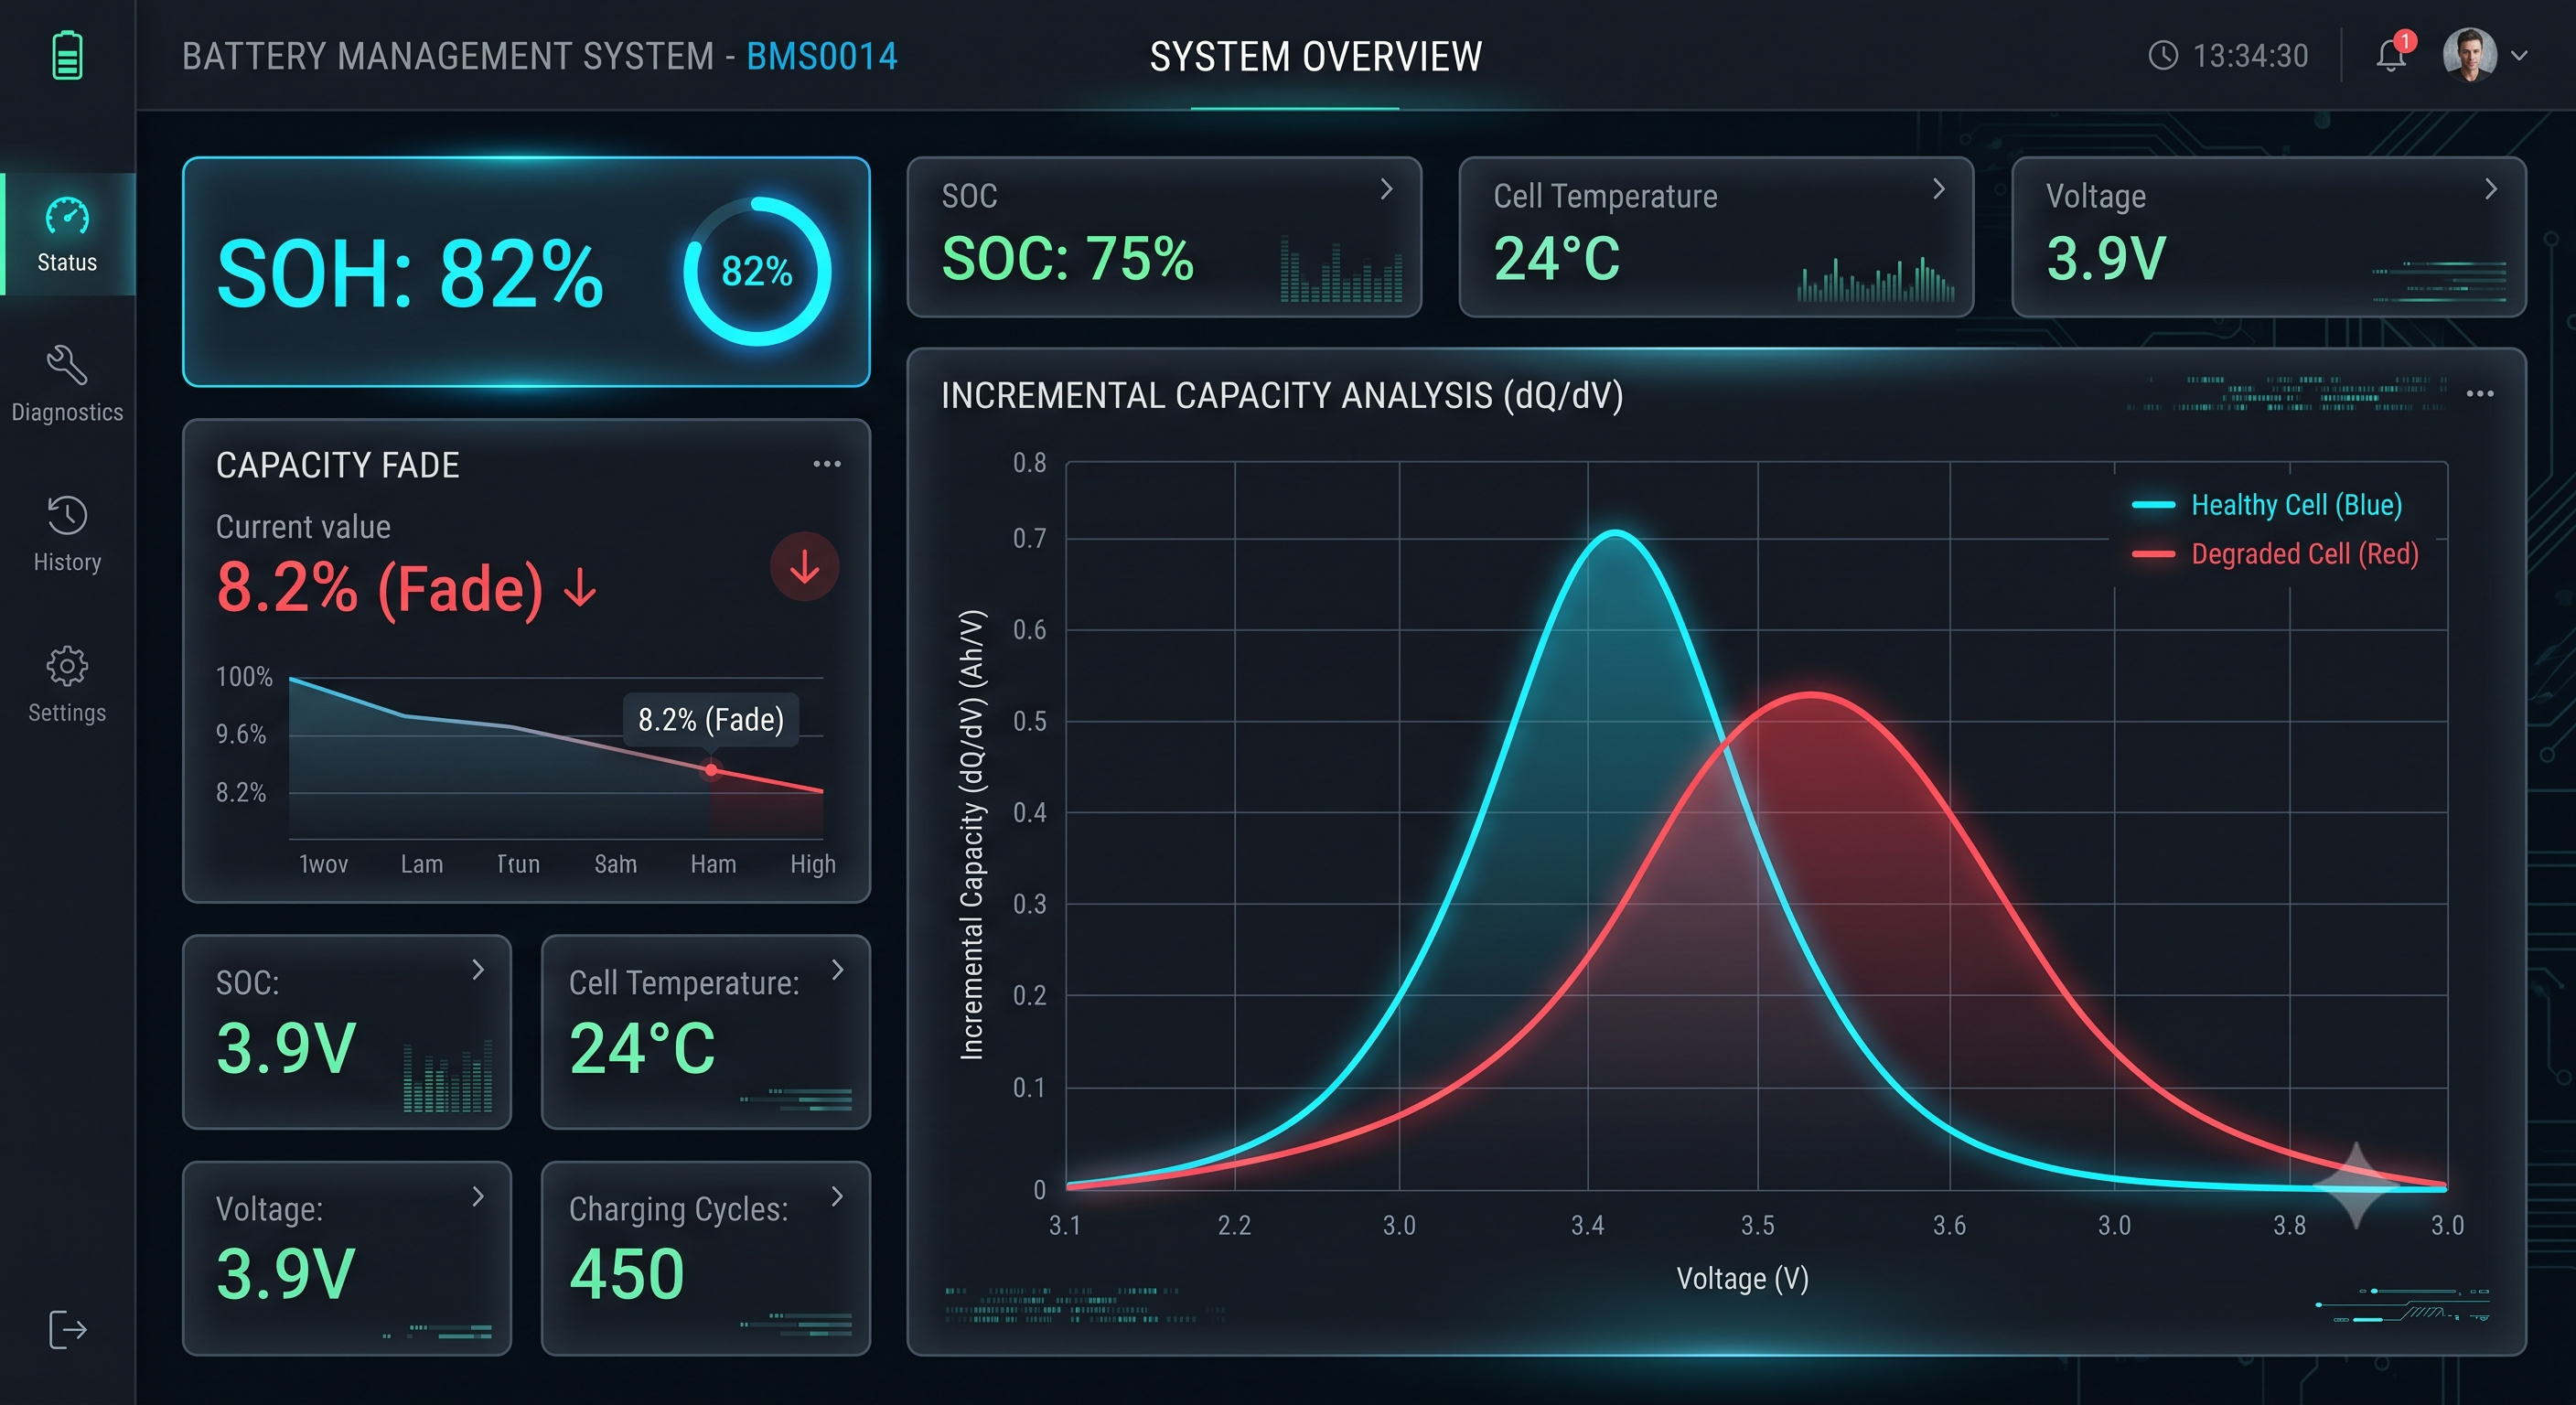
\includegraphics[width=0.65\textwidth]{last9.png}
\label{fig:13_smoothing_placeholder}
\end{figure}

% ============================================================
\section{Remaining Useful Life (RUL) Prediction}
\label{sec:13_rul}

Estimating the \emph{current} SOH answers the question "how healthy is the battery today?" A related, and from a fleet-operations and warranty perspective often more valuable, question is "how much longer will this battery remain usable?" — the Remaining Useful Life problem.

\subsection{Problem Definition}
\label{subsec:13_rul_definition}

RUL is typically defined as the remaining time (or remaining equivalent full cycles, or remaining throughput) until the battery's $SOH_C$ crosses the predefined end-of-life threshold discussed in Section~\ref{subsec:13_sohc} (commonly 70–80\%):
\begin{equation}
    \text{RUL}(t) = \inf \left\{ \tau > 0 : SOH_C(t + \tau) \le SOH_{C,\text{EOL}} \right\}
    \label{eq:13_rul_definition}
\end{equation}
Because the future trajectory of $SOH_C$ depends on future usage patterns that are not known in advance (how the vehicle will be driven, charged, and stored going forward), RUL prediction is fundamentally a forecasting problem under uncertainty, not merely an extrapolation of a deterministic curve.

\subsection{Model-Based Extrapolation}
\label{subsec:13_rul_model_based}

The simplest RUL approach projects the fitted empirical fade model of Section~\ref{sec:13_fade_models} forward in time, assuming that future usage statistically resembles historical usage (same average temperature, DoD, and throughput rate). This approach is computationally cheap and easy to communicate to a vehicle owner as a single number, but, as discussed in Section~\ref{subsec:13_knee_point}, it can substantially misestimate RUL for cells approaching a knee point, since the pre-knee fade model has no mechanism to anticipate the coming acceleration.

\subsection{Particle-Filter-Based RUL with Uncertainty Bounds}
\label{subsec:13_rul_particle_filter}

A more sophisticated approach, increasingly common in prognostics research and in higher-end commercial fleet-management platforms, represents the uncertain future fade trajectory as a distribution over many candidate trajectories (a "particle" population), each propagated forward using a (possibly randomly perturbed) fade model, and weighted according to how well each particle's past trajectory matches the observed SOH history. This particle-filter approach naturally produces not just a single point estimate of RUL, but a full probability distribution — allowing the BMS or fleet dashboard to report, for example, "80\% confidence the battery will remain above 80\% SOH for at least 6 more years" rather than a single potentially over-precise number. The computational cost of maintaining and propagating a particle population is nontrivial, and in most current production systems this calculation is performed off-vehicle, in the cloud, using periodically uploaded SOH history rather than onboard the vehicle's real-time microcontroller.



% ============================================================
\section{Summary}
\label{sec:13_summary}

State of Health tracking is a critical function that prevents sudden battery failure and ensures the ongoing accuracy of State of Charge estimators. Because physical degradation mechanisms — such as SEI layer growth, lithium plating, particle micro-cracking, transition metal dissolution, and conductivity loss — cannot be measured directly, SOH must be inferred mathematically, and its evolution is shaped by four dominant stress factors: temperature, storage SOC, depth of discharge, and C-rate.

Empirical calendar- and cycle-aging models provide a physically-motivated baseline expectation for how capacity and resistance should evolve over time, though these models must be used cautiously near the nonlinear "knee point" that many cells exhibit late in life. The Dual-Time-Scale Extended Kalman Filter resolves the numerical instability of estimating fast states and slow parameters simultaneously, provided the input data contains sufficient persistent excitation to make the slow parameters observable. Differential techniques like Incremental Capacity Analysis and Differential Voltage Analysis translate everyday (or periodically scheduled) charging curves into deep electrochemical diagnostics, capable in principle of distinguishing specific degradation modes, though practical deployment requires careful smoothing and controlled excitation conditions. Finally, Remaining Useful Life prediction extends point-in-time SOH estimation into a forward-looking, uncertainty-aware forecast, of direct value to fleet operators, warranty programs, and vehicle owners alike.

Tracking these shifting parameters over years of operation sets the stage for Chapter~14, where we will scale these concepts up from a single cell to a multi-cell battery pack, and confront the reality that no two cells in that pack will age identically.

% ============================================================
  

% ============================================================
% AI IMAGE GENERATION PROMPTS
% ============================================================
% If you wish to include realistic visualizations for this chapter,
% use the following prompts in an AI image generator (like Midjourney):
%
% PROMPT 1 (For Section 13.2 - SEI Layer / Micro-cracking):
% "A highly detailed, 3D microscopic scientific illustration of a 
% lithium-ion battery anode. Show spherical graphite particles with 
% glowing lithium ions. The surface of the particles should be covered 
% in a thick, rough, crystalline crust representing the Solid Electrolyte 
% Interphase (SEI) layer. Include subtle micro-cracks in the graphite. 
% Blue and dark gray color palette, electron microscope aesthetic."
%
% PROMPT 2 (For Section 13.2.1 - Lithium Plating / Dendrite Growth):
% "A dramatic macro scientific illustration of a lithium-ion battery 
% anode surface during fast charging at low temperature, showing 
% needle-like metallic lithium dendrites growing outward from the 
% graphite surface toward a thin separator membrane. Warning-style 
% amber and silver color palette, high technical detail, cutaway 
% cross-section view."
%
% PROMPT 3 (For Section 13.3 - Stress Factor Sensitivity Panels):
% "A clean scientific data-visualization illustration composed of four 
% small line-graph panels arranged in a grid, each showing a degradation 
% curve rising with a different stress factor: temperature, storage 
% state of charge, depth of discharge, and charge rate. Minimalist 
% engineering report style, muted blue and orange color palette."
%
% PROMPT 4 (For Section 13.4 - Knee Point Behavior):
% "A minimalist technical line-chart illustration on a white background 
% showing a battery capacity retention curve that declines gently and 
% linearly for most of its length, then bends sharply downward near the 
% end, with a small circular marker and dashed vertical line labeled 
% 'knee point' at the bend. Clean vector engineering-report style."
%
% PROMPT 5 (For Section 13.5 - Data Diagnostics Dashboard):
% "A modern, dark-themed UI dashboard for a Battery Management System. 
% The screen displays a complex 'Incremental Capacity' bell curve graph, 
% comparing a healthy blue curve with a degraded, shifted red curve. 
% The interface includes technical readouts for 'SOH: 82%' and 'Capacity 
% Fade'. Futuristic, clean, data-driven visualization."
%
% PROMPT 6 (For Section 13.6 - Remaining Useful Life Fan Chart):
% "A polished analytics dashboard illustration showing a Remaining 
% Useful Life forecast chart: a solid line trending downward representing 
% historical battery health, transitioning into a widening shaded cone 
% of uncertainty representing future projections, with a horizontal 
% dashed red line marking the end-of-life threshold. Dark theme, 
% futuristic fleet-management software aesthetic."
% ============================================================